\documentclass[a4paper, 10.5pt, oneside]{report} %book format on A4 paper with size 12 font

%------------PREAMBLE
\input{preamble}
\usepackage{morefloats}
%---------------------------
                                          
\begin{document}

%---------------------------TITLE PAGE
\include{cover}

%---------------------------ABSTRACT
\begin{abstract}
This report investigates self-organized criticality in the Bak--Tang--Wiesenfeld sandpile model. The model is simulated on a finite two-dimensional lattice, where grains are added slowly and unstable sites topple by distributing grains to their nearest neighbours. Open boundaries allow grains to leave the system, making the model a driven dissipative system. The main observables are the average pile height, avalanche size, avalanche area, avalanche loss, and avalanche length. The average height is used to test whether the system reaches a statistically stationary state, while avalanche distributions are used to test for scale-invariant behaviour. The standard model with uniformly random grain addition is compared with an extended model in which grains are added preferentially near the centre of the lattice. The aim is to determine whether both models display evidence of self-organized criticality and to understand how changing the driving rule affects the avalanche statistics.
\end{abstract}

%---------------------------TABLE OF CONTENTS
\tableofcontents
%---------------------------

%---------------------------MAIN BODY
\chapter{Important definition for report}\label{ch:introduction1}

\section{SOC meaning}\label{sec:socdef}

Self-organized criticality was introduced by Bak, Tang, and Wiesenfeld \cite{bak1987soc,bak1988soc}, usually abbreviated as SOC, describes a class of complex systems that naturally evolve towards a critical state without the need for carefully tuned external parameters. In such systems, small local changes can sometimes produce responses of many different sizes, ranging from negligible events to large-scale avalanches. This means that the size of an event is not necessarily proportional to the size of its cause.

A standard example of SOC is the Bak--Tang--Wiesenfeld sandpile model. In this model, grains of sand are added slowly to a lattice. When the height at a site exceeds a fixed threshold, that site topples and redistributes grains to its neighbours. This redistribution may cause further topplings, producing an avalanche. Although the local rules are simple, the collective behaviour of the system can be highly non-trivial.

A key feature of SOC systems is scale invariance. After the system reaches a statistically stationary state, there is no single characteristic avalanche size. Instead, small avalanches occur frequently, while large avalanches occur more rarely, often following a power-law distribution. This makes the sandpile model a useful framework for studying how complex macroscopic behaviour can arise from simple microscopic rules.

In this chapter, we introduce the idea of SOC and use the sandpile model as a simple computational example. The goal is to investigate how repeated local interactions can drive the system towards a critical state, and how avalanche statistics can be used to identify scale-invariant behaviour.

\section{BTW-model Notation}\label{sec:btwmodeldef}

Let the sandpile be defined on an $N\times M$ rectangular lattice. Write
\[
    h_t(i,j)
\]
for the number of grains at site $(i,j)$ after the $t$-th grain addition, where
\[
    1\leq i\leq N,\qquad 1\leq j\leq M.
\]
A site $(i,j)$ is called \emph{unstable} if
\[
    h_t(i,j)\geq 4.
\]
When an unstable site topples, its height decreases by $4$, and each of its four nearest neighbours receives one grain:
\[
    h(i,j)\mapsto h(i,j)-4,
\]
\[
    h(i\pm 1,j)\mapsto h(i\pm 1,j)+1,
    \qquad
    h(i,j\pm 1)\mapsto h(i,j\pm 1)+1.
\]
If a grain is sent outside the boundary of the lattice, then it is lost from the system.

\section*{Question 1}

\textbf{Why is it that a system exhibiting scale invariance will have phenomena which are described by a power law?}

Let $s$ denote the size of an event. For example, in the sandpile model, $s$ may denote the number of topplings in an avalanche. Let $P(s)$ denote the frequency or probability distribution of events of size $s$.

Scale invariance means that if we rescale the event size by a positive constant factor $a>0$, the distribution should have the same shape, up to an overall multiplicative factor. That is, we expect
\[
    P(as)=C(a)P(s),
\]
where $C(a)$ depends only on the scaling factor $a$, not on $s$.

A function satisfying this kind of scaling relation is a power law. Suppose
\[
    P(s)=Cs^{-\alpha},
\]
where $C>0$ and $\alpha>0$ are constants. Then
\[
    P(as)=C(as)^{-\alpha}
    =Ca^{-\alpha}s^{-\alpha}
    =a^{-\alpha}P(s).
\]
Thus, after rescaling $s\mapsto as$, the distribution is changed only by the multiplicative constant $a^{-\alpha}$, while the functional form is unchanged.

Therefore, if a system has no characteristic event-size scale, then the natural form of its event-size distribution is
\[
    P(s)\propto s^{-\alpha}.
\]
This explains why scale-invariant systems are commonly associated with power-law distributions. In the BTW sandpile model, this means that avalanche sizes may occur over a wide range of scales, with small avalanches being common and large avalanches being rare, but not exponentially rare, this will be seen from the data I collected.

\section*{Question 2}

\textbf{In what ways does the BTW model satisfy the properties required for a system to exhibit self-organized criticality?}

A system exhibiting self-organized criticality usually has the following properties:

\begin{enumerate}[label=(\roman*)]
    \item it is slowly driven;
    \item it has local interactions;
    \item it has dissipation(we lose the quantity that is been slowly added);
    \item it evolves toward a critical state without fine-tuning of external parameters;
    \item it produces avalanches over many different scales.
\end{enumerate}

The BTW model satisfies these properties as follows.

\subsection*{Slow driving}

At each time step, only one grain of sand is added to the lattice. Hence the system is driven slowly and locally. The system is not forced by a large global perturbation \footnote{It should be said that this is within the realm of what uuually happens and we don’t consider largeperturbations to the syssem (succ as a large meteorite crashing on Earth whicc may ccange the tecconicsdrassically, cause enormous foress ffres, result in epidemicsas the ecosyssem ccanges,and cause the ffnancialmarket to crash as civilization collapses)}. Instead, small local changes gradually build up stress in the system, causing avalanches.

\subsection*{Local interactions}

The toppling is local. When a site $(i,j)$ topples, it only affects its four nearest neighbours:
\[
    (i+1,j),\quad (i-1,j),\quad (i,j+1),\quad (i,j-1).
\]
There are no long-range interactions in the basic model. Therefore, all large-scale behaviour comes from repeated local redistribution of sand.

\subsection*{Dissipation}

The finite boundary of the lattice provides dissipation. If a boundary site topples, then some grains may be sent outside the lattice and are deleted from the system. Thus sand can enter the system through grain addition and leave the system through the boundary.

\subsection*{Self-organization}

No external parameter needs to be tuned to a critical value. Starting from an empty lattice, the average amount of sand initially increases. Eventually, avalanches carry sand to the boundary, where grains are lost. After a transient period, the system reaches a statistically stationary regime where the average input of sand is balanced by the average loss of sand.

\subsection*{Avalanches over many scales}

A single added grain may cause no toppling, a small avalanche, or a very large avalanche. Hence the system produces events over a broad range of sizes. In the critical regime, one expects avalanche statistics to be broad and often approximately described by power laws.

Therefore, the BTW model is a standard example of a self-organized critical system because it is slowly driven, locally interacting, dissipative, and naturally evolves toward a critical state without external fine-tuning.

\section*{Question 3}

\textbf{Why is it important for the table to have finite boundaries? What if we had an infinite lattice, but dropped the sand on only a finite subset of the lattice?}

The finite boundary is important because it allows sand to leave the system. This is the dissipation mechanism of the BTW model.

Define the total amount of sand in the system by
\[
    S_t=\sum_{i=1}^{N}\sum_{j=1}^{M} h_t(i,j).
\]
Each grain addition increases $S_t$ by $1$. Interior topplings conserve the total amount of sand, because the toppling site loses $4$ grains and its four neighbours receive $1$ grain each. Hence the total change from an interior toppling is
\[
    -4+1+1+1+1=0.
\]
However, boundary topplings can decrease $S_t$, because some grains are sent outside the lattice and are deleted. Therefore, in a long-time statistically stationary state, we expect the average input rate to balance the average dissipation rate:
\[
    \text{average sand input rate}
    =
    \text{average sand loss rate}.
\]
Since one grain is added per time step, the average loss rate should also approach one grain per time step in the stationary regime.

If the lattice were infinite, there would be no boundary where sand could be lost. If sand were dropped only on a finite subset of an infinite lattice, then the local region might still generate avalanches, but the total amount of sand in the infinite system would keep increasing because no grains are deleted. Sand could spread farther and farther away, but it would not leave the system.

Thus, an infinite lattice lacks the same dissipative mechanism. Without dissipation, the model is no longer the same open driven-dissipative system. Consequently, it is not clear that it would reach the same kind of statistically stationary SOC state as the finite-boundary BTW model.

Hence finite boundaries are important because they make the BTW model an open system:
\[
    \text{sand enters by driving}
    \quad\text{and}\quad
    \text{sand leaves through the boundary}.
\]

\section*{Question 4}

\textbf{Without simulating anything, what might you expect the average height to be once the system has reached a steady state? Compare your initial expectation to what your simulation does.}

The average height is defined by
\[
    \langle h_t\rangle
    :=
    \frac{1}{NM}\sum_{i=1}^{N}\sum_{j=1}^{M}h_t(i,j).
\]

A stable site must satisfy
\[
    h_t(i,j)<4.
\]
Therefore, the possible stable heights are
\[
    h_t(i,j)\in\{0,1,2,3\}.
\]

A first naive expectation is that the stable heights $0,1,2,3$ might occur equally often. If this were true, then the average height would be
\[
    \langle h\rangle_{\mathrm{naive}}
    =
    \frac{0+1+2+3}{4}
    =
    \frac{3}{2}.
\]
So a very simple first guess is
\[
    \langle h\rangle\approx 1.5.
\]

However, this assumption is too naive. The recurrent configurations of the BTW model are not uniformly distributed over all stable configurations. The system tends to organize itself near a critical state, where many sites are close to becoming unstable. Therefore, heights $2$ and $3$ should occur more frequently than a uniform distribution would suggest.

Thus a more realistic expectation is
\[
    1.5<\langle h\rangle<4.
\]
For the standard two-dimensional BTW model with open boundaries and a large lattice, one typically expects the long-time average height to be around
\[
    \langle h\rangle \approx 2.1\text{--}2.2.
\]

In simulation, one should expect the following behaviour. Starting from an empty lattice,
\[
    \langle h_0\rangle=0.
\]
As grains are added, $\langle h_t\rangle$ initially increases. After sufficiently many grain additions, boundary losses begin to balance input. Then $\langle h_t\rangle$ should not become exactly constant, but should fluctuate around a stable long-time mean:
\[
    \langle h_t\rangle \approx \text{constant in a long-time statistical sense}.
\]

Therefore, the system should reach a statistically stationary average height rather than a perfectly fixed height configuration.

\section*{Question 5}

\textbf{Explain the difference between a steady state, a statistically stationary state, and an equilibrium state. Do you expect the BTW model to reach an equilibrium state or a statistically stationary state? In terms of system observables, how might we characterize this state?}

\subsection*{Steady state}

A steady state means that the state of the system no longer changes in time. For the sandpile, a strict steady state would mean
\[
    h_{t+1}(i,j)=h_t(i,j)
\]
for every site $(i,j)$ and for all sufficiently large $t$.

The BTW model does not reach this kind of strict steady state because grains keep being added and avalanches keep changing the configuration.

\subsection*{Statistically stationary state}

A statistically stationary state means that the microscopic configuration continues to change, but the statistical properties of the system become time-independent.

For example, after a transient period, the following observables may fluctuate around stable long-time values:
\[
    \langle h_t\rangle,
\]
\[
    P(s),
\]
where $P(s)$ is the avalanche-size distribution, and
\[
    \text{average sand loss rate}.
\]

Thus the exact configuration $h_t$ keeps changing, but its statistical behaviour becomes stable.

\subsection*{Equilibrium state}

An equilibrium state usually refers to a closed system that has relaxed to thermodynamic equilibrium. In equilibrium, there is typically no net flux of mass or energy through the system, and the system often satisfies detailed balance.

The BTW model is not an equilibrium system. It is continuously driven by grain addition and continuously dissipates sand through the boundary. Therefore, it has a nonzero flux:
\[
    \text{input by grain addition}
    \longrightarrow
    \text{redistribution by avalanches}
    \longrightarrow
    \text{loss through boundary}.
\]

Hence the BTW model is a non-equilibrium driven-dissipative system.

\subsection*{Expected state of the BTW model}

The BTW model is expected to reach a statistically stationary state, not an equilibrium state. In this state, the microscopic configuration keeps changing, but long-time statistical observables stabilize.

We may characterize this statistically stationary state using observables such as:
\[
    \langle h_t\rangle
    =
    \frac{1}{NM}\sum_{i=1}^{N}\sum_{j=1}^{M}h_t(i,j),
\]
\[
    P(s),
\]
where $s$ is the number of topplings in an avalanche,
\[
    P(A),
\]
where $A$ is the number of distinct toppled sites,
\[
    P(L),
\]
where $L$ is the amount of sand lost at the boundary, and also a chosen avalanche length observable.

In the statistically stationary SOC regime, we expect the average height to fluctuate around a long-time mean, while avalanche observables have stable long-time distributions. In particular, the avalanche-size distribution may approximately satisfy a power-law relation of the form
\[
    P(s)\propto s^{-\alpha}
\]
for some exponent $\alpha>0$ over an appropriate scaling range.


\chapter{Important notation for testing}\label{ch:introduction2}

\section{Statistic Variable used for the report}\label{sec:vardef}
For the important statistics fetch, we will consider the following properties:
\begin{enumerate}[label=(\roman*)]
	\item Topples: The number of topples required to take the grid from its initial unstable configuration to a stable one;
	\item Area: The number of unique sites which have been toppled;
	\item Loss: The number of grains of sand whicc are toppled off the lattice; and,
	\item I define the avalanche length using the Manhattan distance. If the grain is added at \(x_0=(i_0,j_0)\), and \(A\) is the set of sites which topple during the avalanche, then

\[
\ell
=
\max_{(i,j)\in A}
\left(
|i-i_0|+|j-j_0|
\right).
\]

This measures the largest number of horizontal and vertical lattice steps between the avalanche origin and any toppled site. I use the Manhattan distance
because topplings in the BTW model only send grains to the four nearest neighbours, not diagonally. Therefore the Manhattan distance matches the geometry of the toppling rule.
\end{enumerate}


\section*{Question 6}

\textbf{Is there a difference between sampling a syssem over time andsampling an ensemble of syssems? If so, under what circumssances? Hint: Look up the property of ergodicity and argue whether or not you believe thebtw model is ergodic.}

There is a difference between sampling a system over time and sampling an ensemble of systems.

Sampling a system over time means running one sandpile simulation for a long time and recording avalanche observables after the system has reached its statistically stationary state. For example, if \(A_t\) is an avalanche observable at time \(t\), such as the number of topples or the avalanche area, then the time average is

\[
\overline{A}_{\mathrm{time}}
=
\frac{1}{T}
\sum_{t=1}^{T} A_t .
\]

On the other hand, sampling an ensemble of systems means running many independent simulations, usually with different random seeds or different initial conditions, and averaging the same observable over these different systems. If there are \(M\) independent simulations and \(A^{(m)}\) is the observable measured in the \(m\)-th simulation, then the ensemble average is

\[
\overline{A}_{\mathrm{ensemble}}
=
\frac{1}{M}
\sum_{m=1}^{M} A^{(m)} .
\]

These two averages are not always the same. They are expected to agree only if the system is ergodic. A system is ergodic if a sufficiently long time average taken from one typical trajectory is equal to the ensemble average over many independent systems. In other words, for an observable \(A\), ergodicity means

\[
\lim_{T\to\infty}
\frac{1}{T}
\sum_{t=1}^{T} A_t
=
\mathbb{E}[A],
\]

where \(\mathbb{E}[A]\) denotes the ensemble expectation of \(A\).

For the BTW sandpile model, I expect the system to be approximately ergodic after the initial transient period has been removed. The reason is that grains are added randomly, and the random driving causes the system to move through many different stable configurations. Therefore, a sufficiently long simulation should sample the statistically stationary state reasonably well.

However, in a finite simulation this agreement is only approximate. The measured avalanche statistics may depend on the lattice size, the number of grain additions, and the length of the transient period. Rare large avalanches may not occur often enough in a short simulation, so the time average from one run may differ from the ensemble average over many independent runs.

Therefore, in this project, I treat a long-time sample from one simulation, after removing the transient period, as an approximation to the statistically stationary ensemble. To improve reliability, one can also run several independent simulations with different random seeds and compare their avalanche distributions.
\chapter{Property of sandpile model}\label{ch:introduction3}

\section{Q7 Avalanche Distributions}

\textbf{Record the frequency with which avalanches have a specific number of topples, area, loss and length. What kind of distribution do you get for each? If possible, can you find a fit for the distribution? (E.g. for a Gaussian, find the mean and width of the distribution; for a power law, find the exponent.)}

Question 7 asks us to record the frequency with which avalanches have a specific number of topples, area, loss and length, and to determine what kind of distribution is obtained for
each quantity. In the Bak--Tang--Wiesenfeld model, an avalanche is produced after adding
one grain of sand to the lattice and then repeatedly toppling unstable sites until the system
returns to a stable configuration.

In this simulation, I used a \(50 \times 50\) lattice and ran the model for \(10^5\) grain additions. No transient cutoff was applied, so avalanches were recorded from the beginning of the simulation. The random seed was fixed at \(41\), and grains were added using a uniform random distribution over the lattice sites.
As discussed in Section~\ref{sec:vardef}, the avalanche variables are defined before analysing their distributions.

\subsection{Histogram Results}

The ordinary histograms are shown in Figure~\ref{fig:q7_histograms}. They are strongly
right-skewed. In all four cases, small avalanches occur very frequently, while large avalanches
are much rarer. This already suggests that the distributions are not Gaussian. A Gaussian
distribution would be concentrated around a typical scale, whereas these avalanche
distributions contain many small events together with some rare but much larger events.

\begin{figure}[htbp]
    \centering

    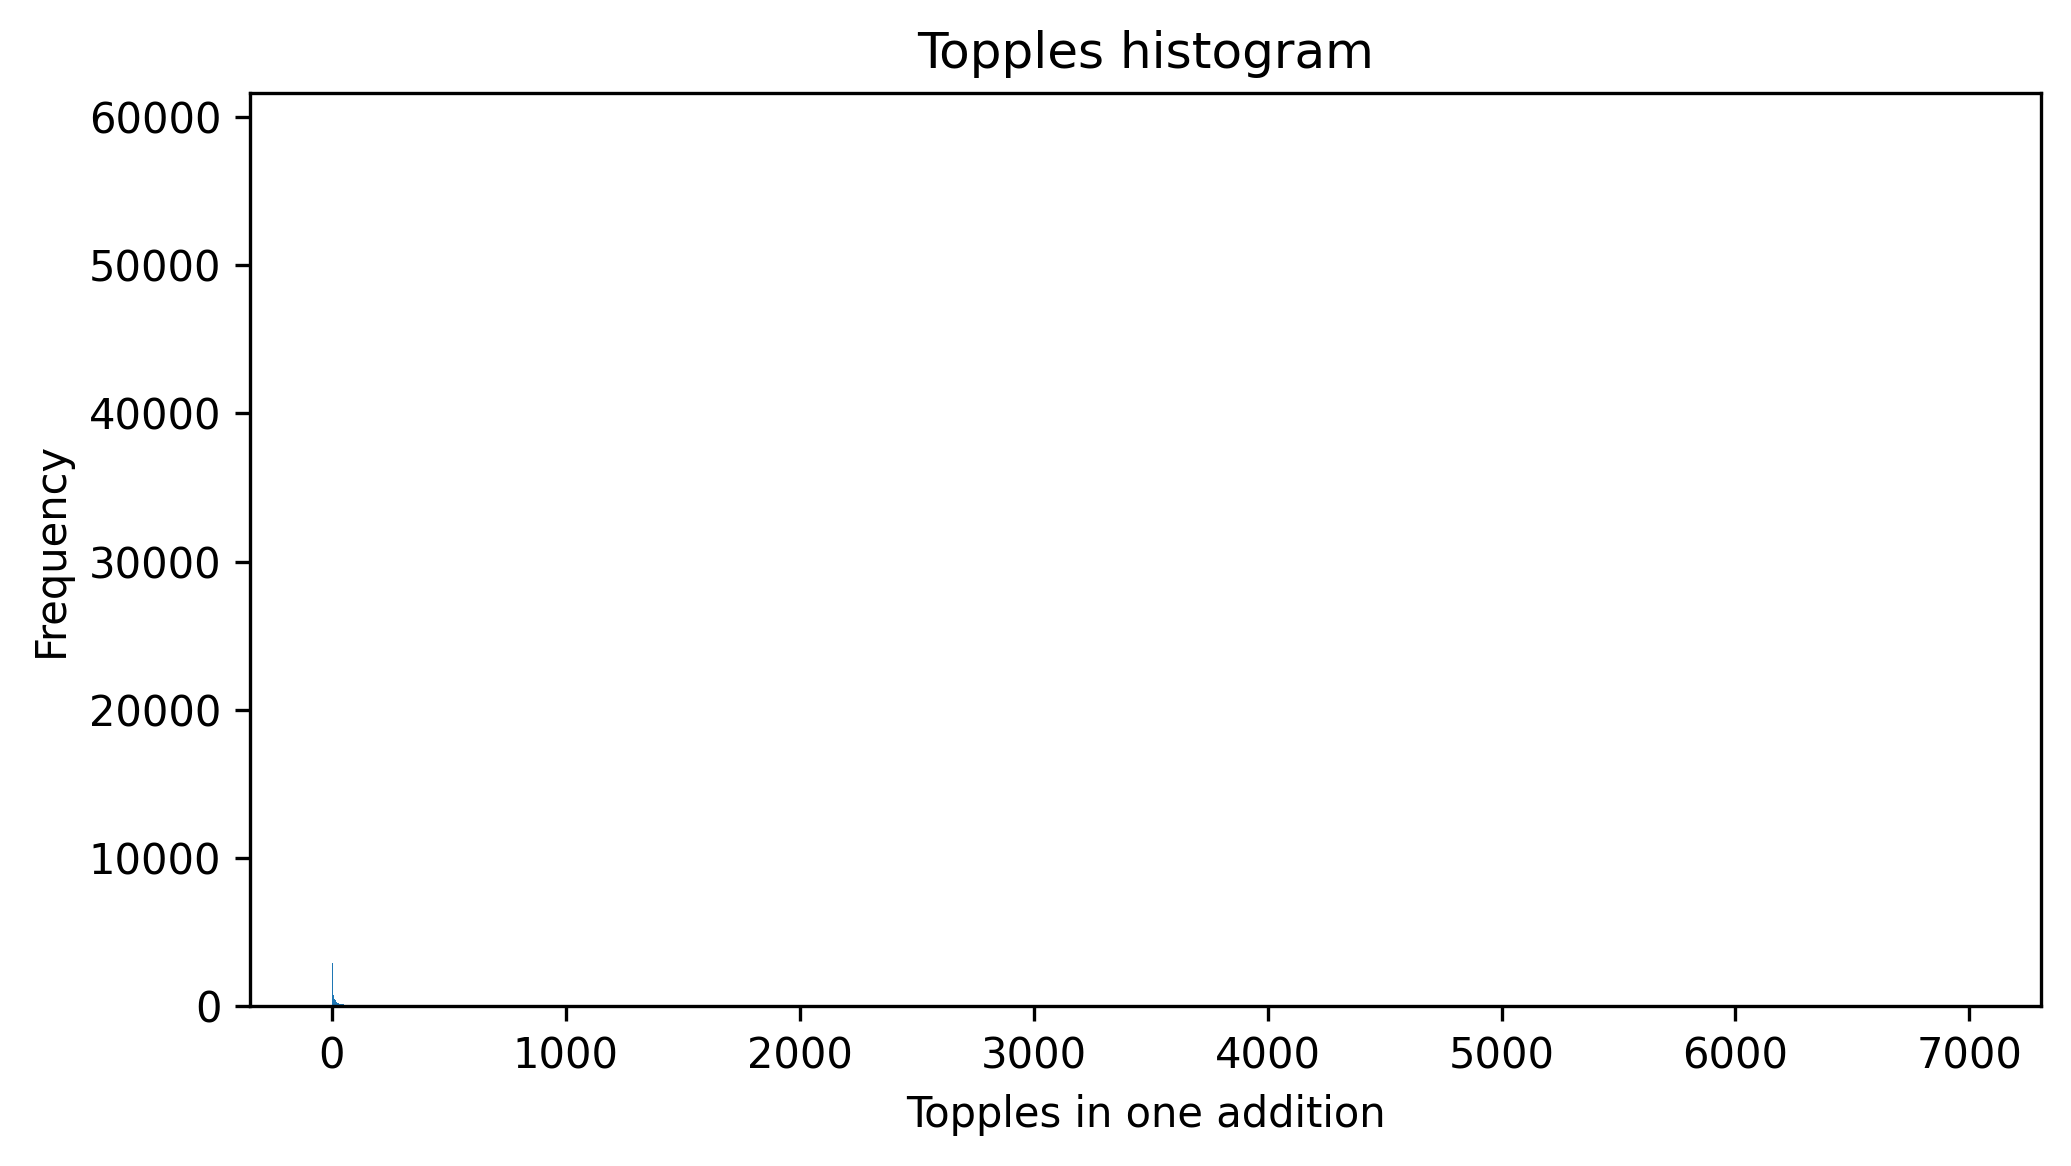
\includegraphics[width=0.45\textwidth]{figures/topple_histogram.png}
    \hfill
    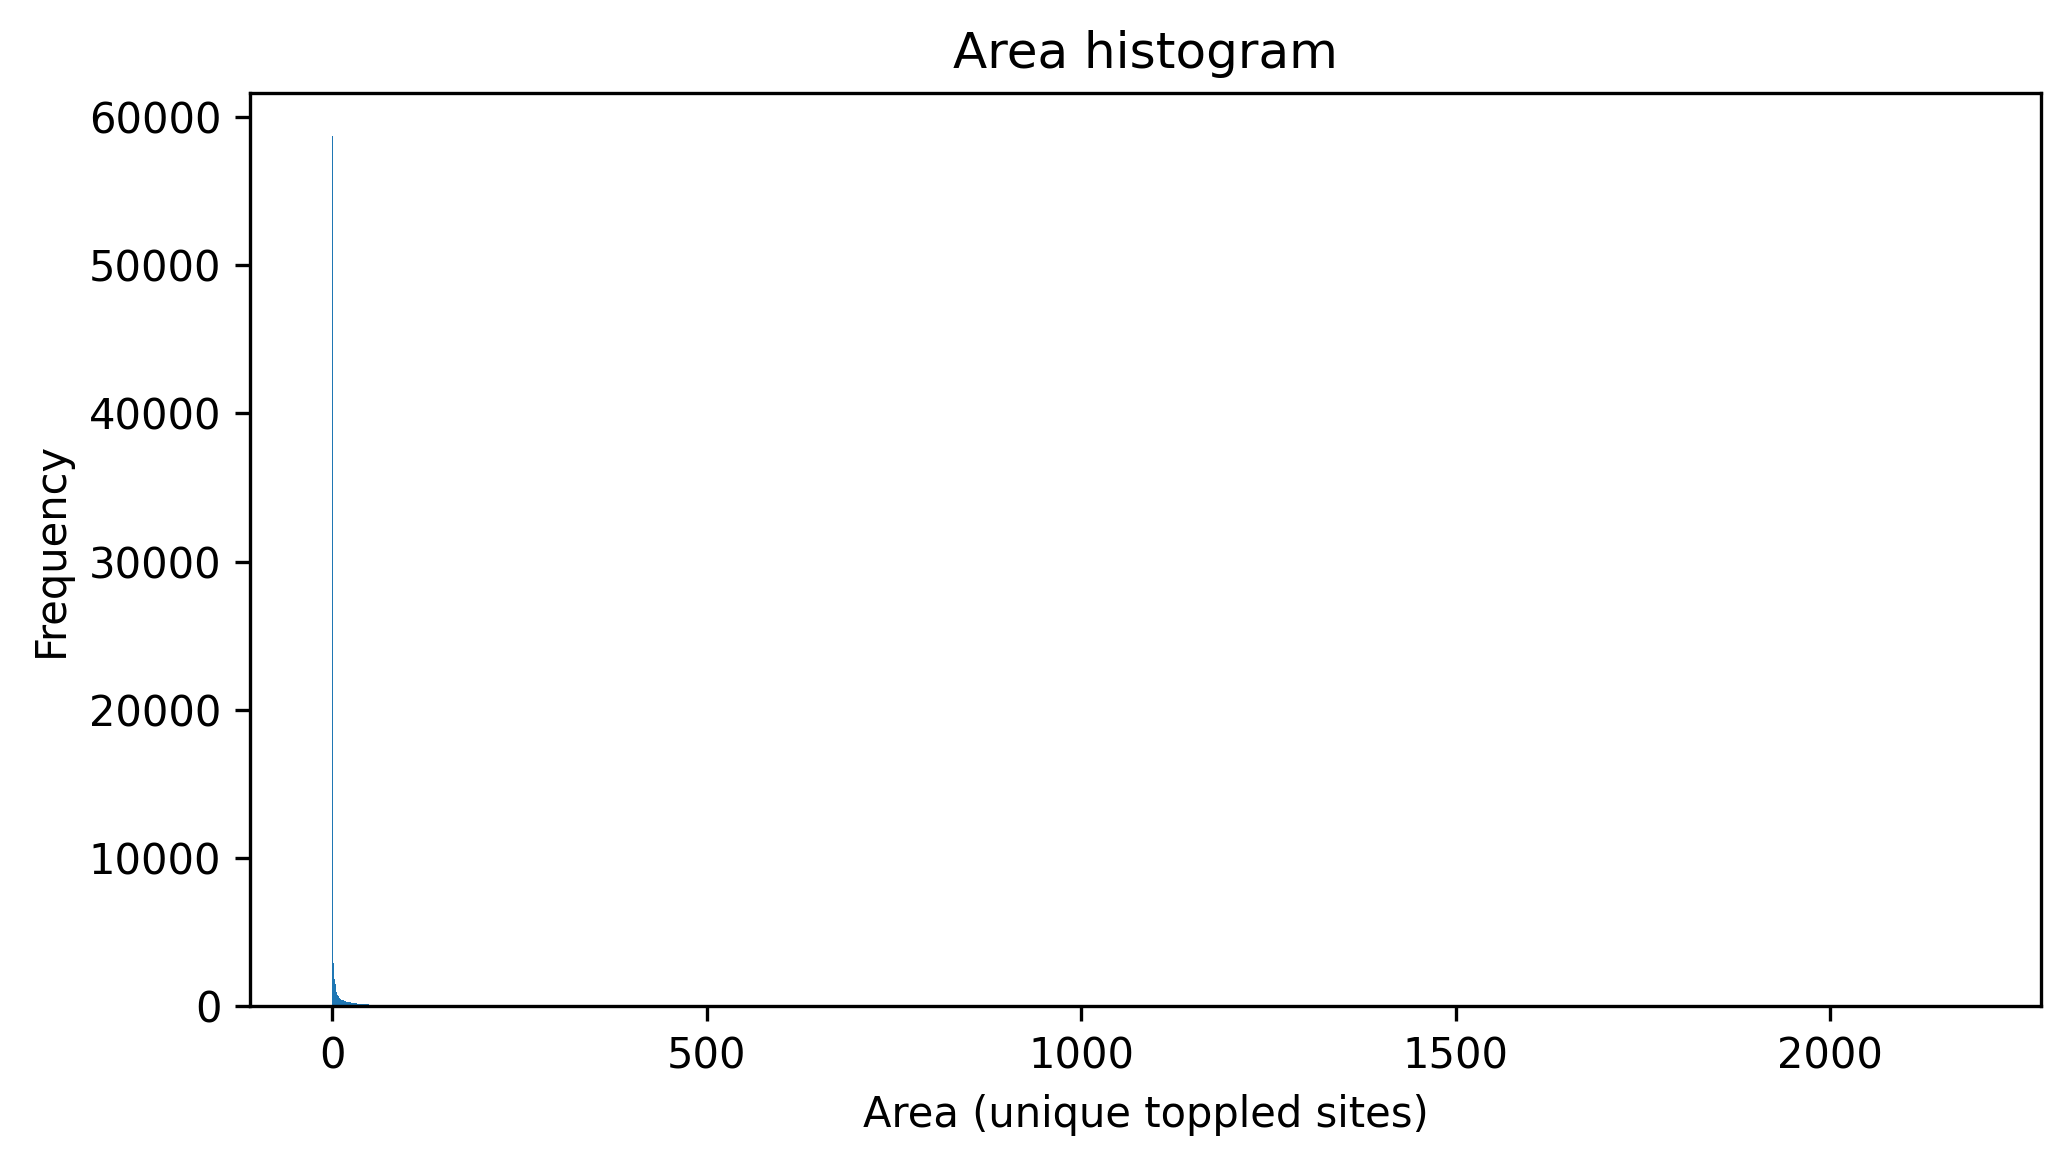
\includegraphics[width=0.45\textwidth]{figures/area_histogram.png}

    \vspace{0.4cm}

    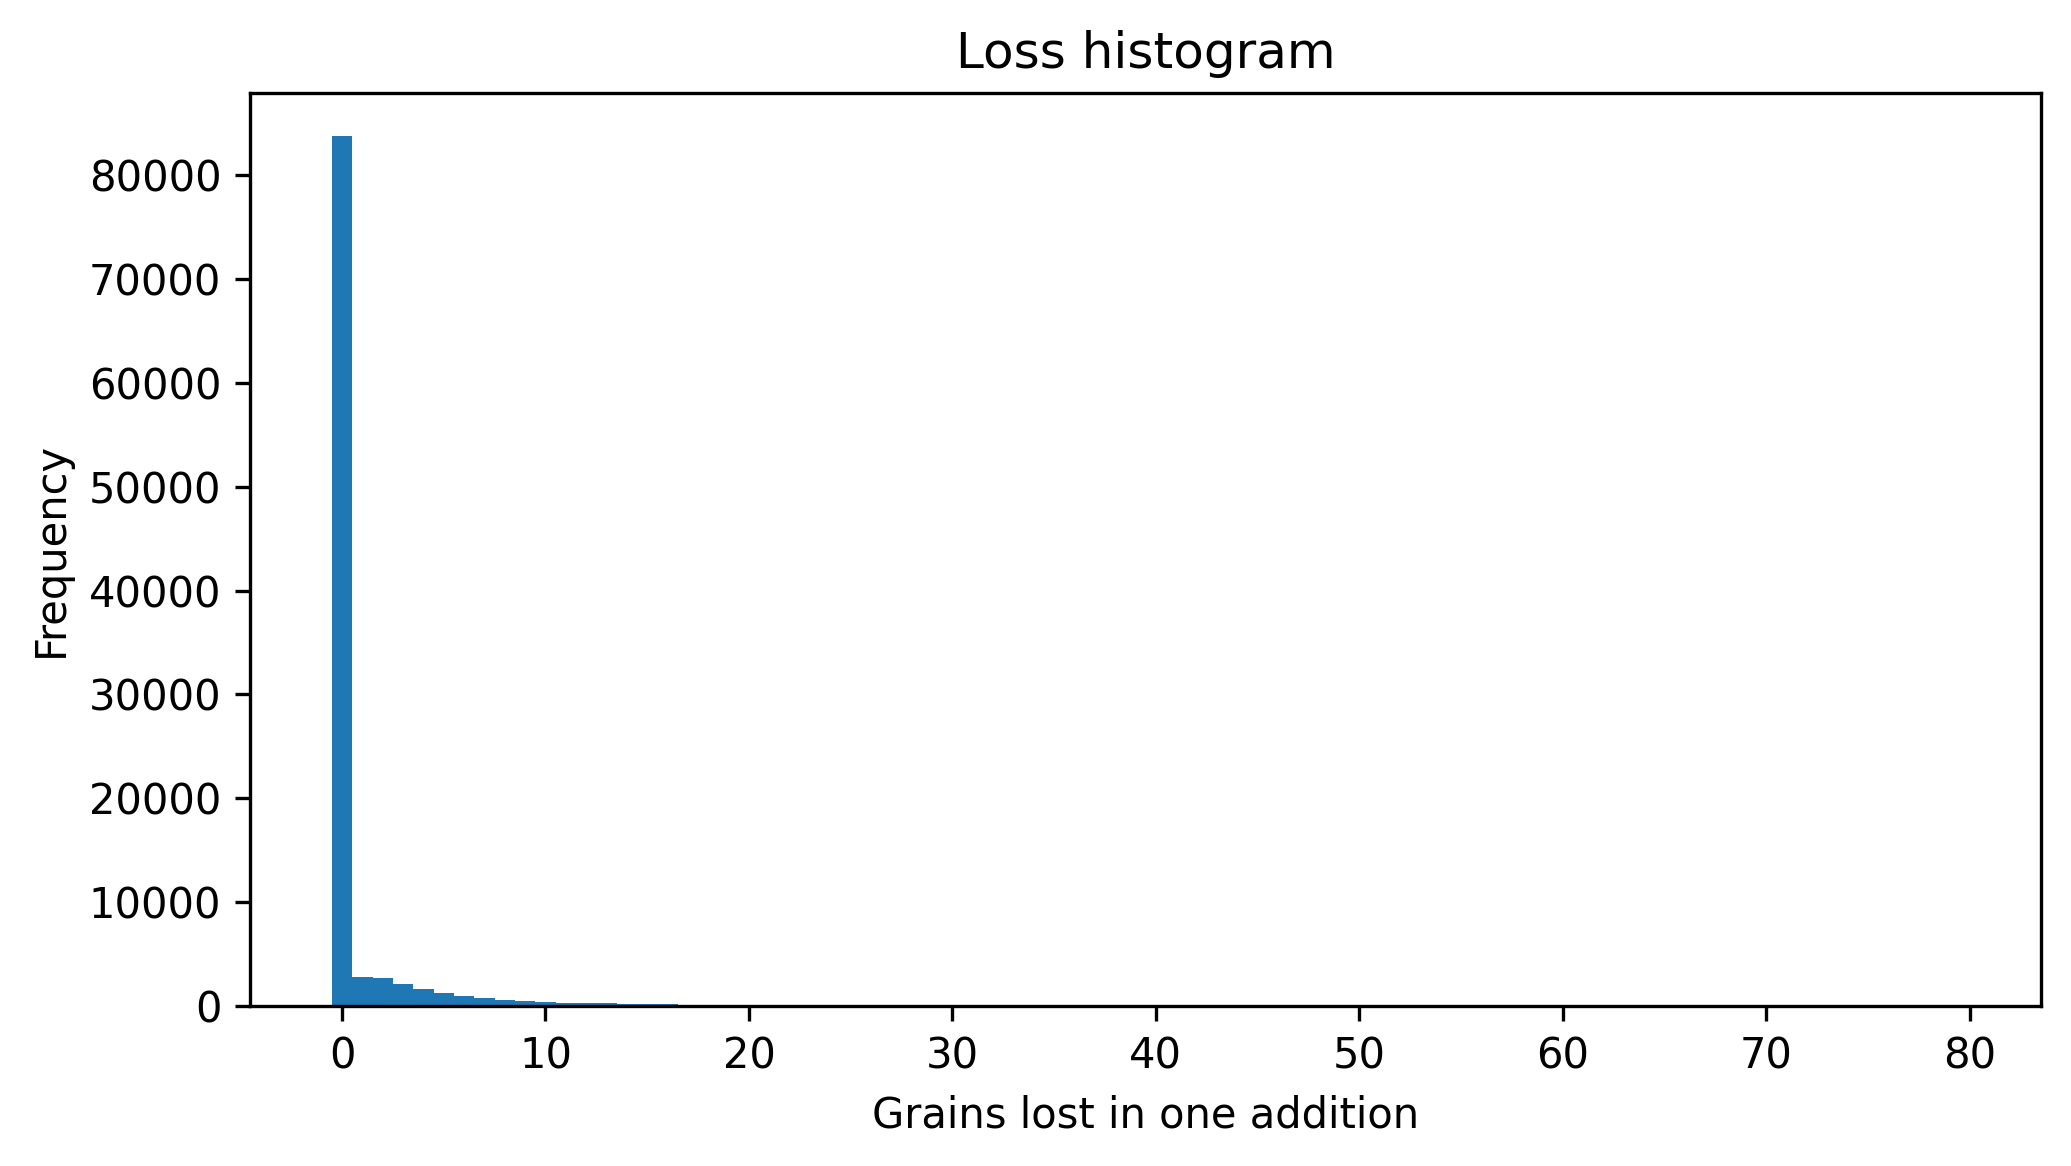
\includegraphics[width=0.45\textwidth]{figures/loss_histogram.png}
    \hfill
    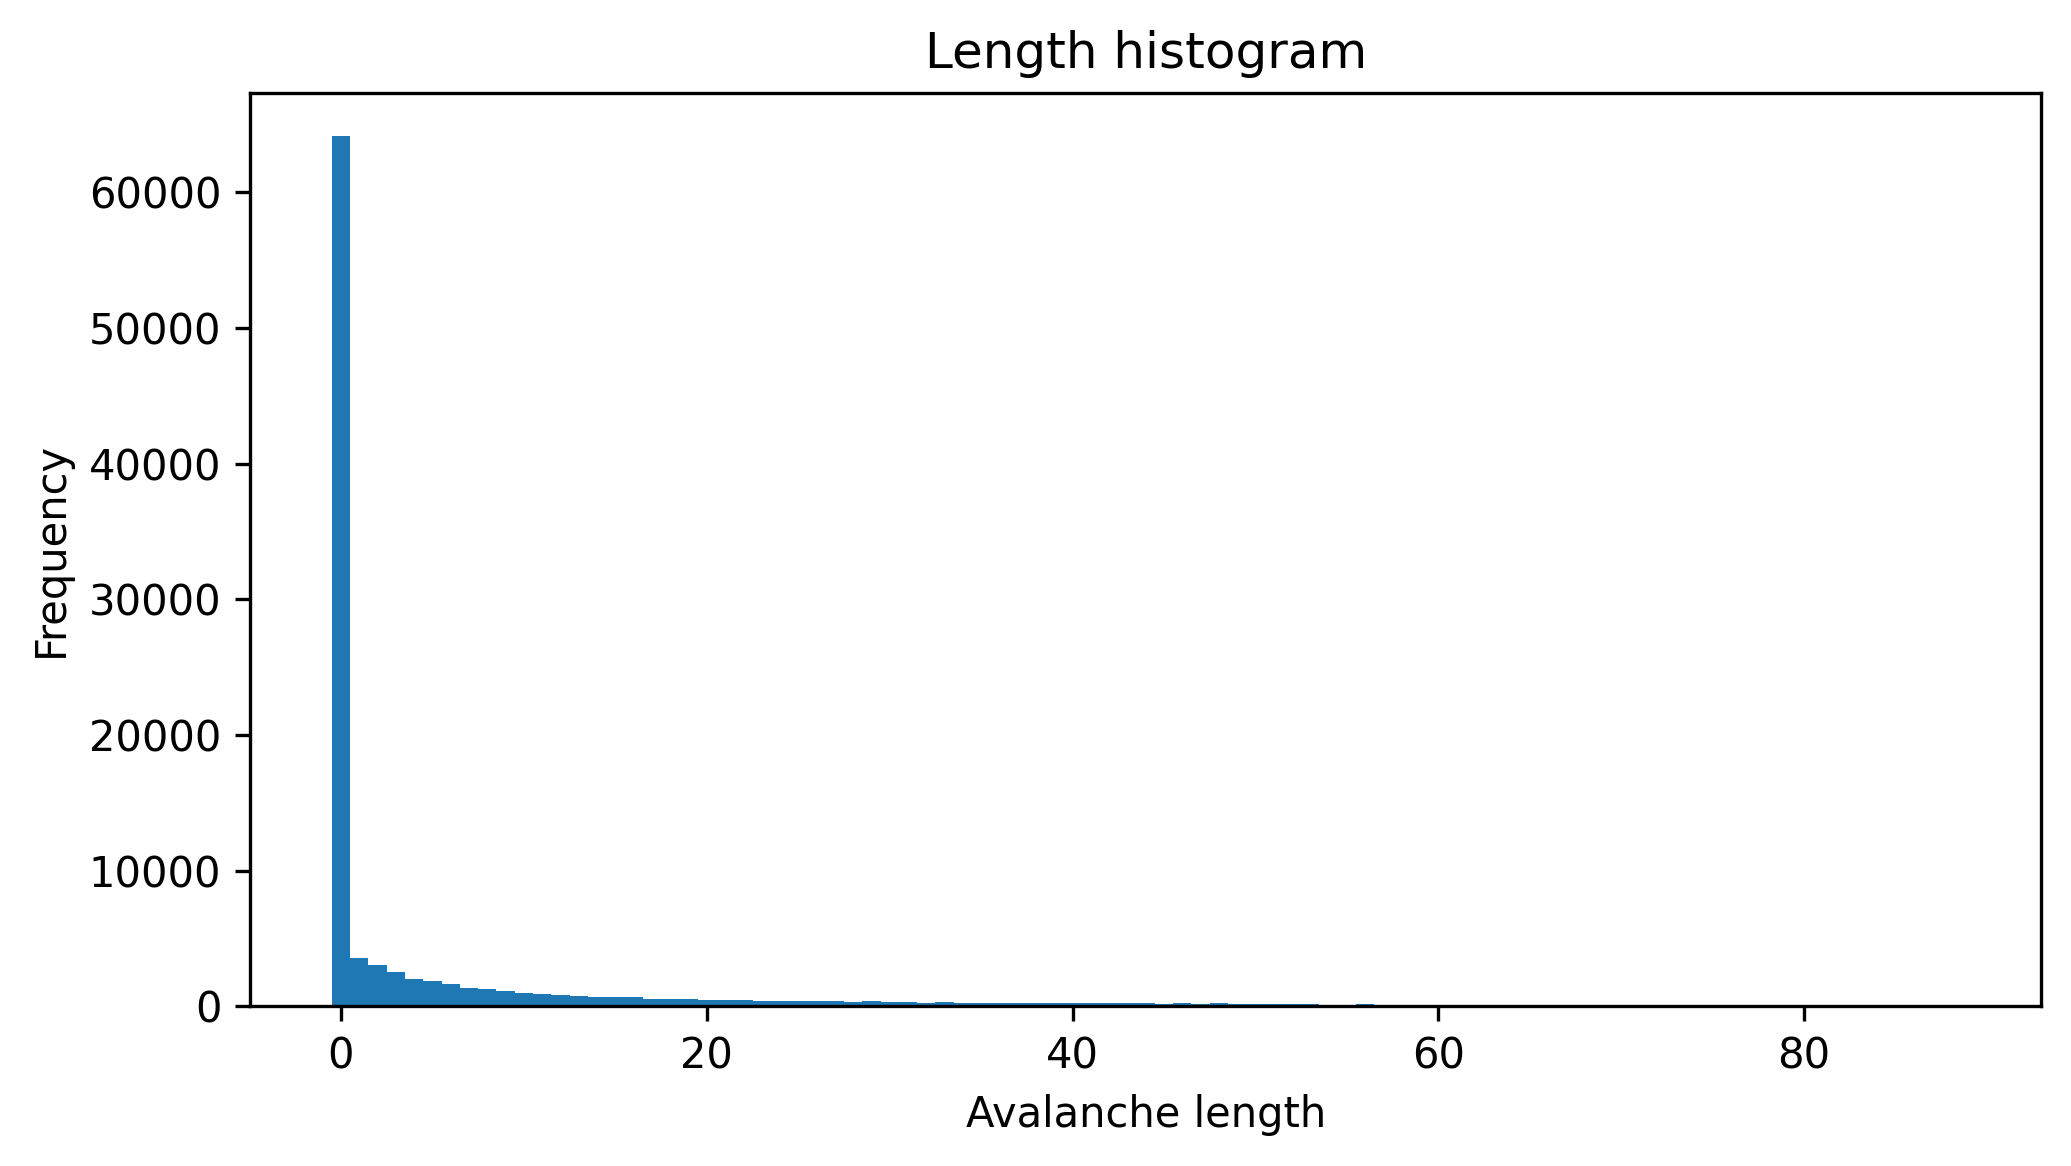
\includegraphics[width=0.45\textwidth]{figures/length_histogram.png}

    \caption{Histograms of avalanche topples, area, loss and length. The distributions are
    strongly right-skewed, with many small avalanches and relatively few large avalanches.}
    \label{fig:q7_histograms}
\end{figure}

\subsection{Log--log Plots and Power-law Behaviour}

To test whether the distributions are approximately power-law distributed, I plotted the
frequency data on log--log axes. A power-law distribution has the form
\[
P(x) \sim Cx^{-\alpha},
\]
where \(x\) is the avalanche observable and \(\alpha\) is the power-law exponent. Taking
logarithms gives
\[
\log P(x) = \log C - \alpha \log x.
\]
Therefore, if the distribution follows a power law, the log--log plot should be approximately
linear, with slope \(-\alpha\).

The log--log plots are shown in Figure~\ref{fig:q7_loglog}. The plots for topples and area
show the clearest approximately linear regions, suggesting that these two quantities are
approximately power-law distributed over an intermediate range. This is consistent with
self-organized criticality: there is no single characteristic avalanche size, and avalanches
occur over a wide range of scales.

\begin{figure}[htbp]
    \centering

    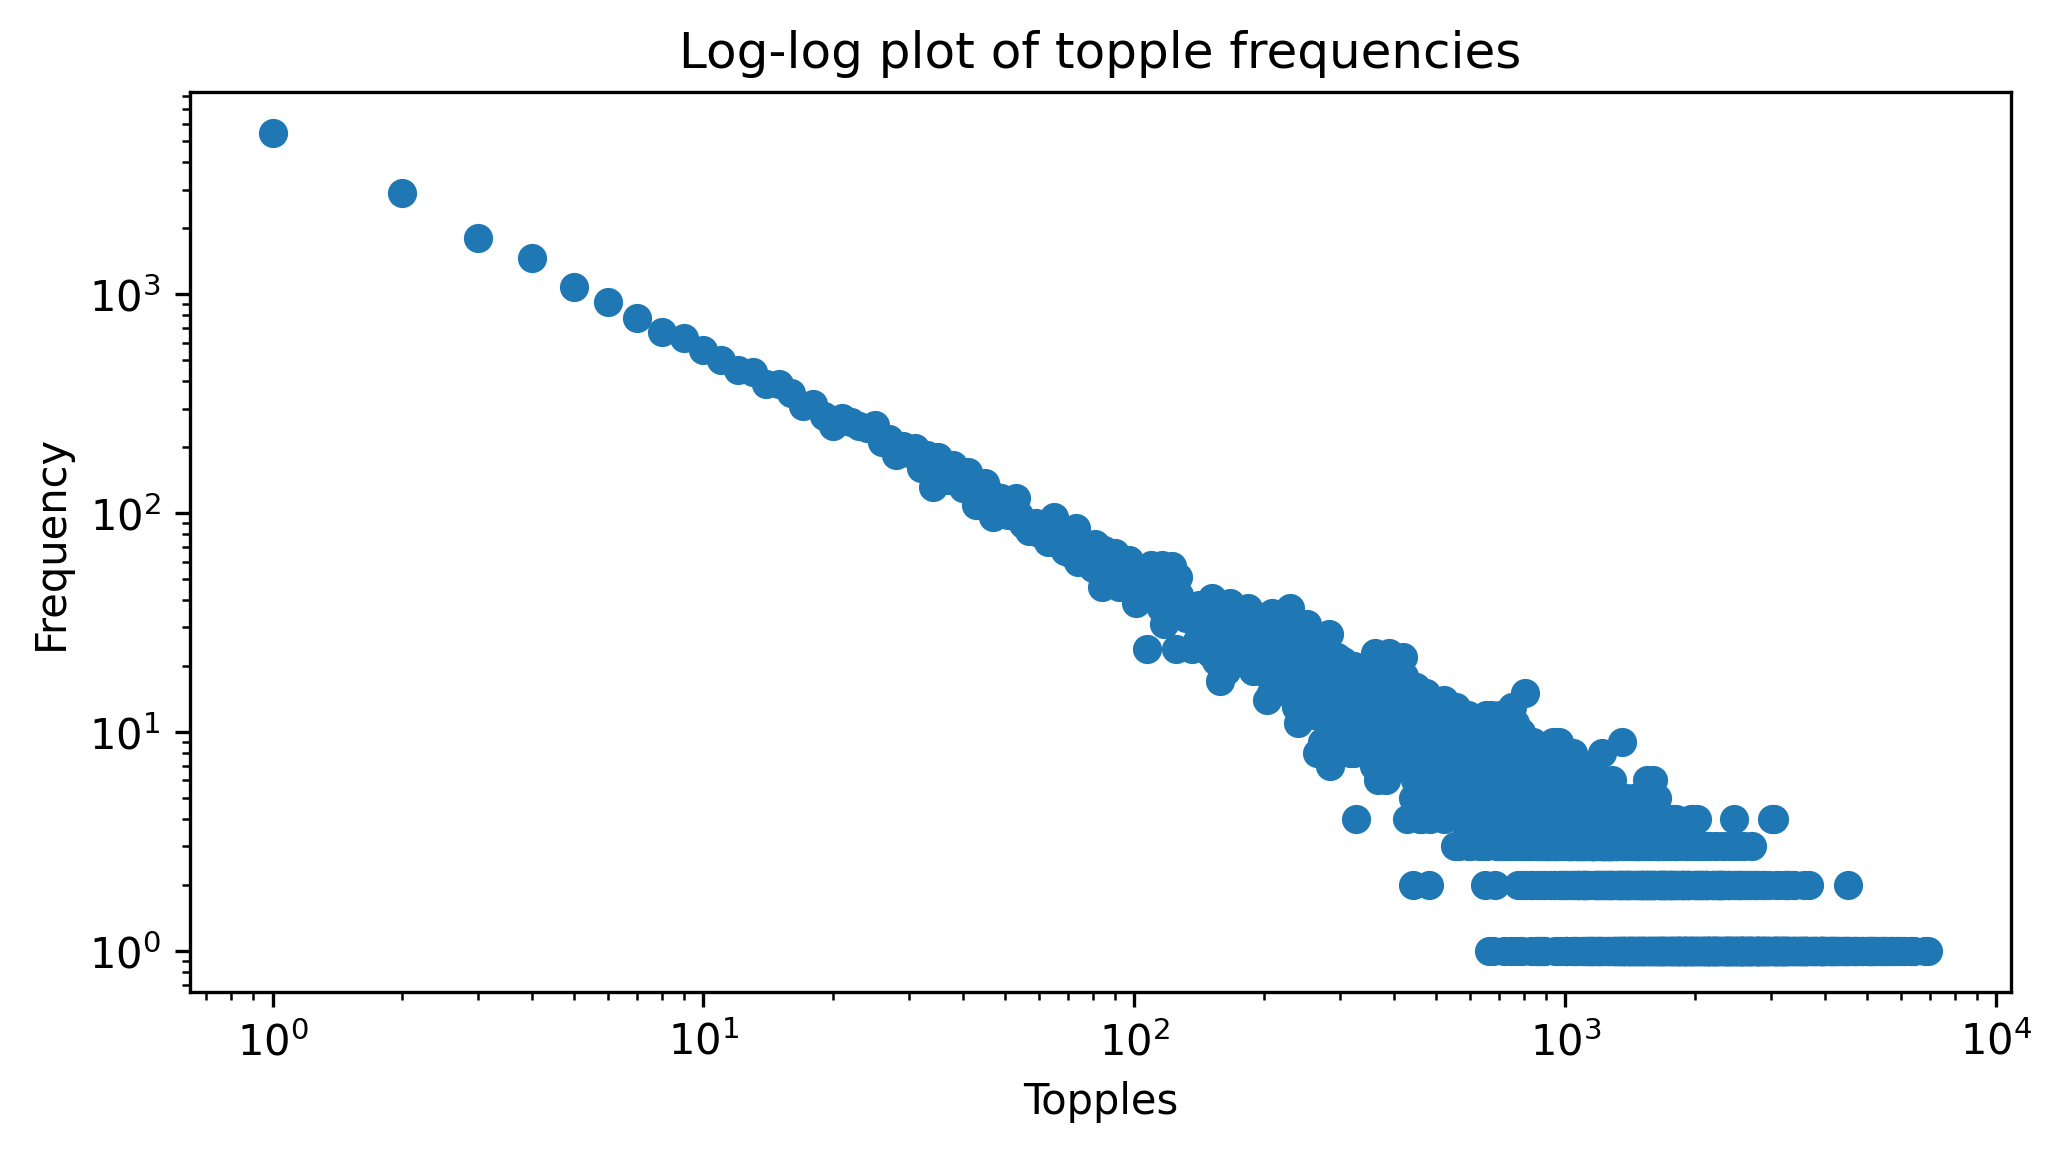
\includegraphics[width=0.45\textwidth]{figures/topple_loglog.png}
    \hfill
    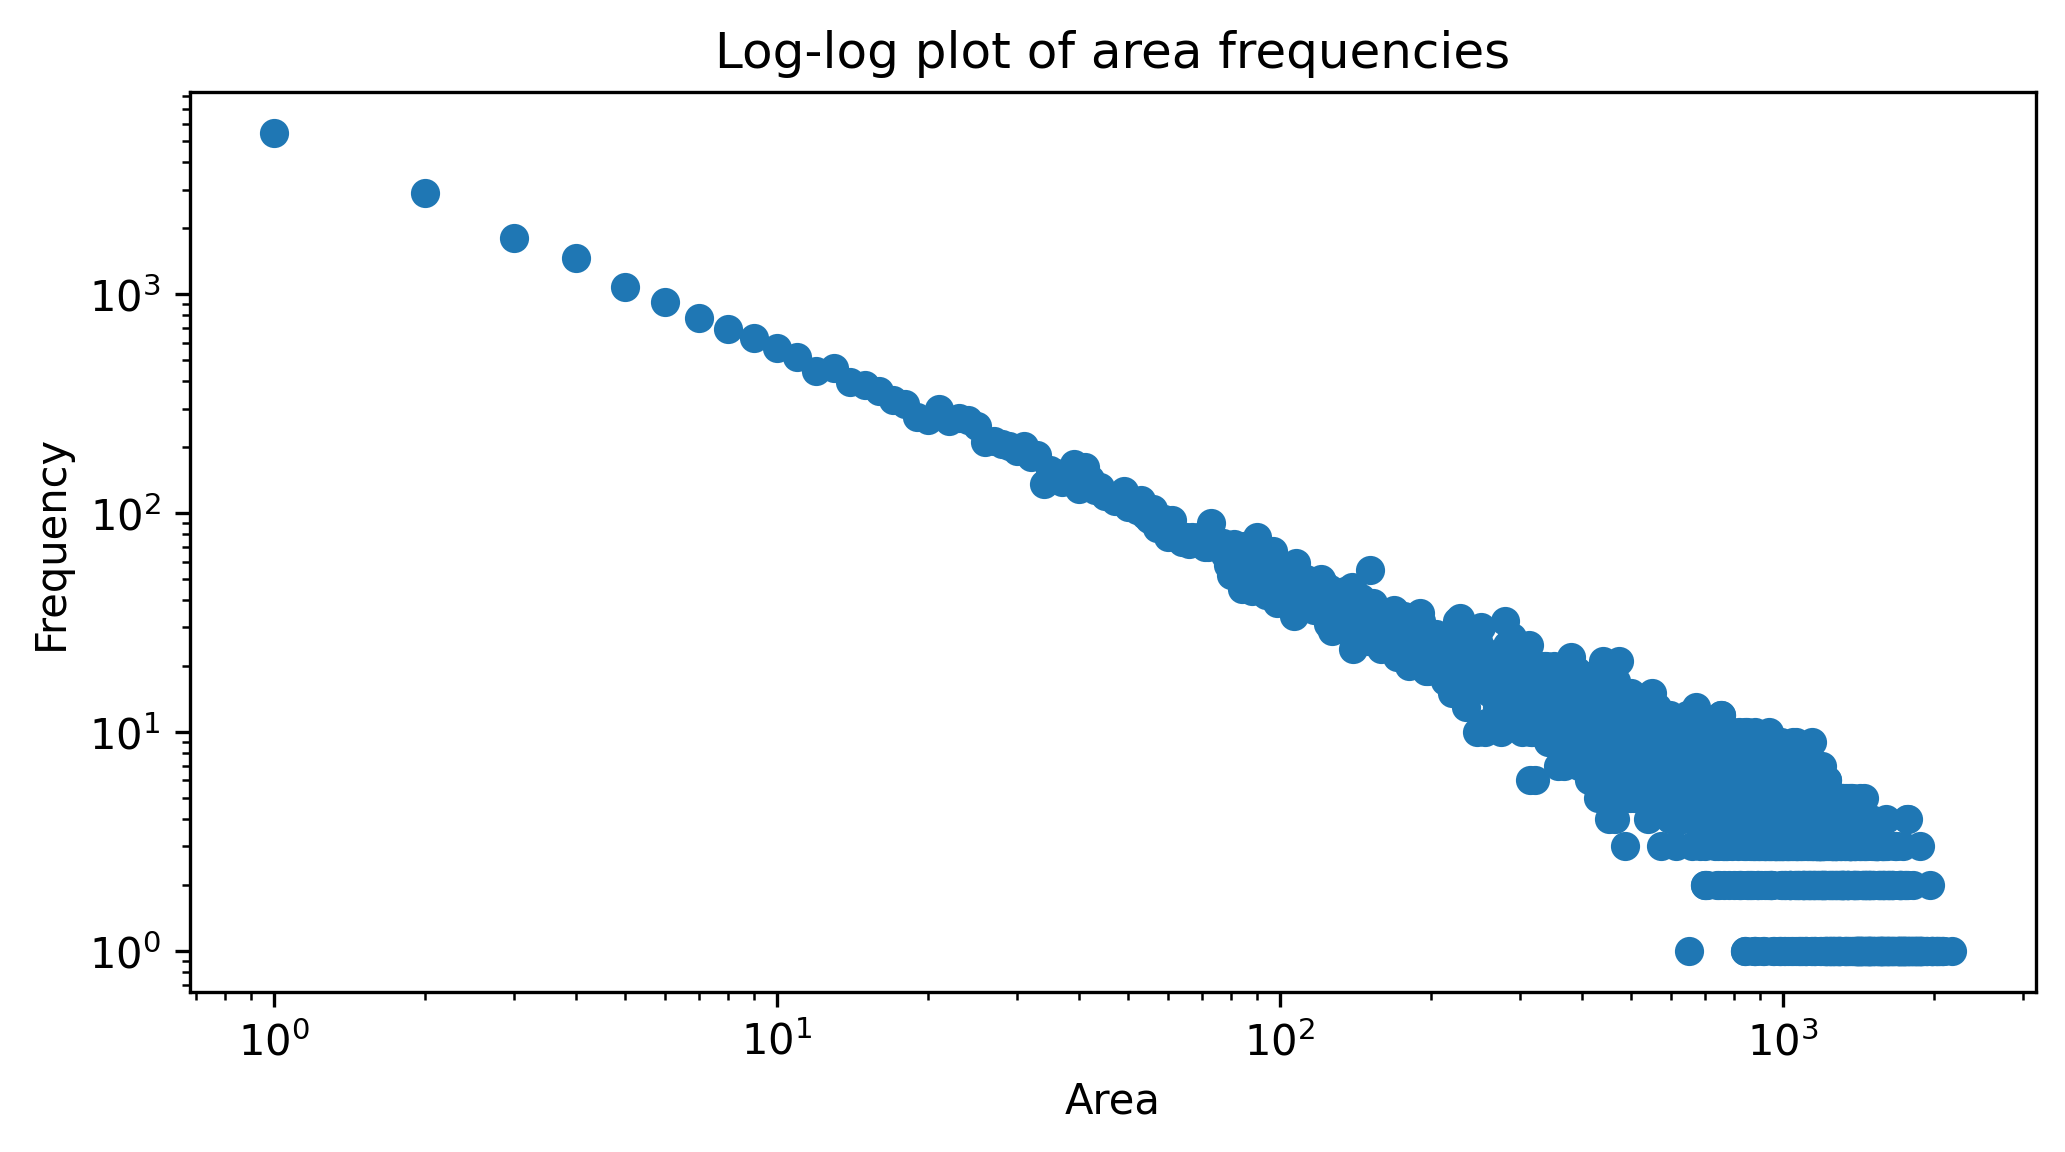
\includegraphics[width=0.45\textwidth]{figures/area_loglog.png}

    \vspace{0.4cm}

    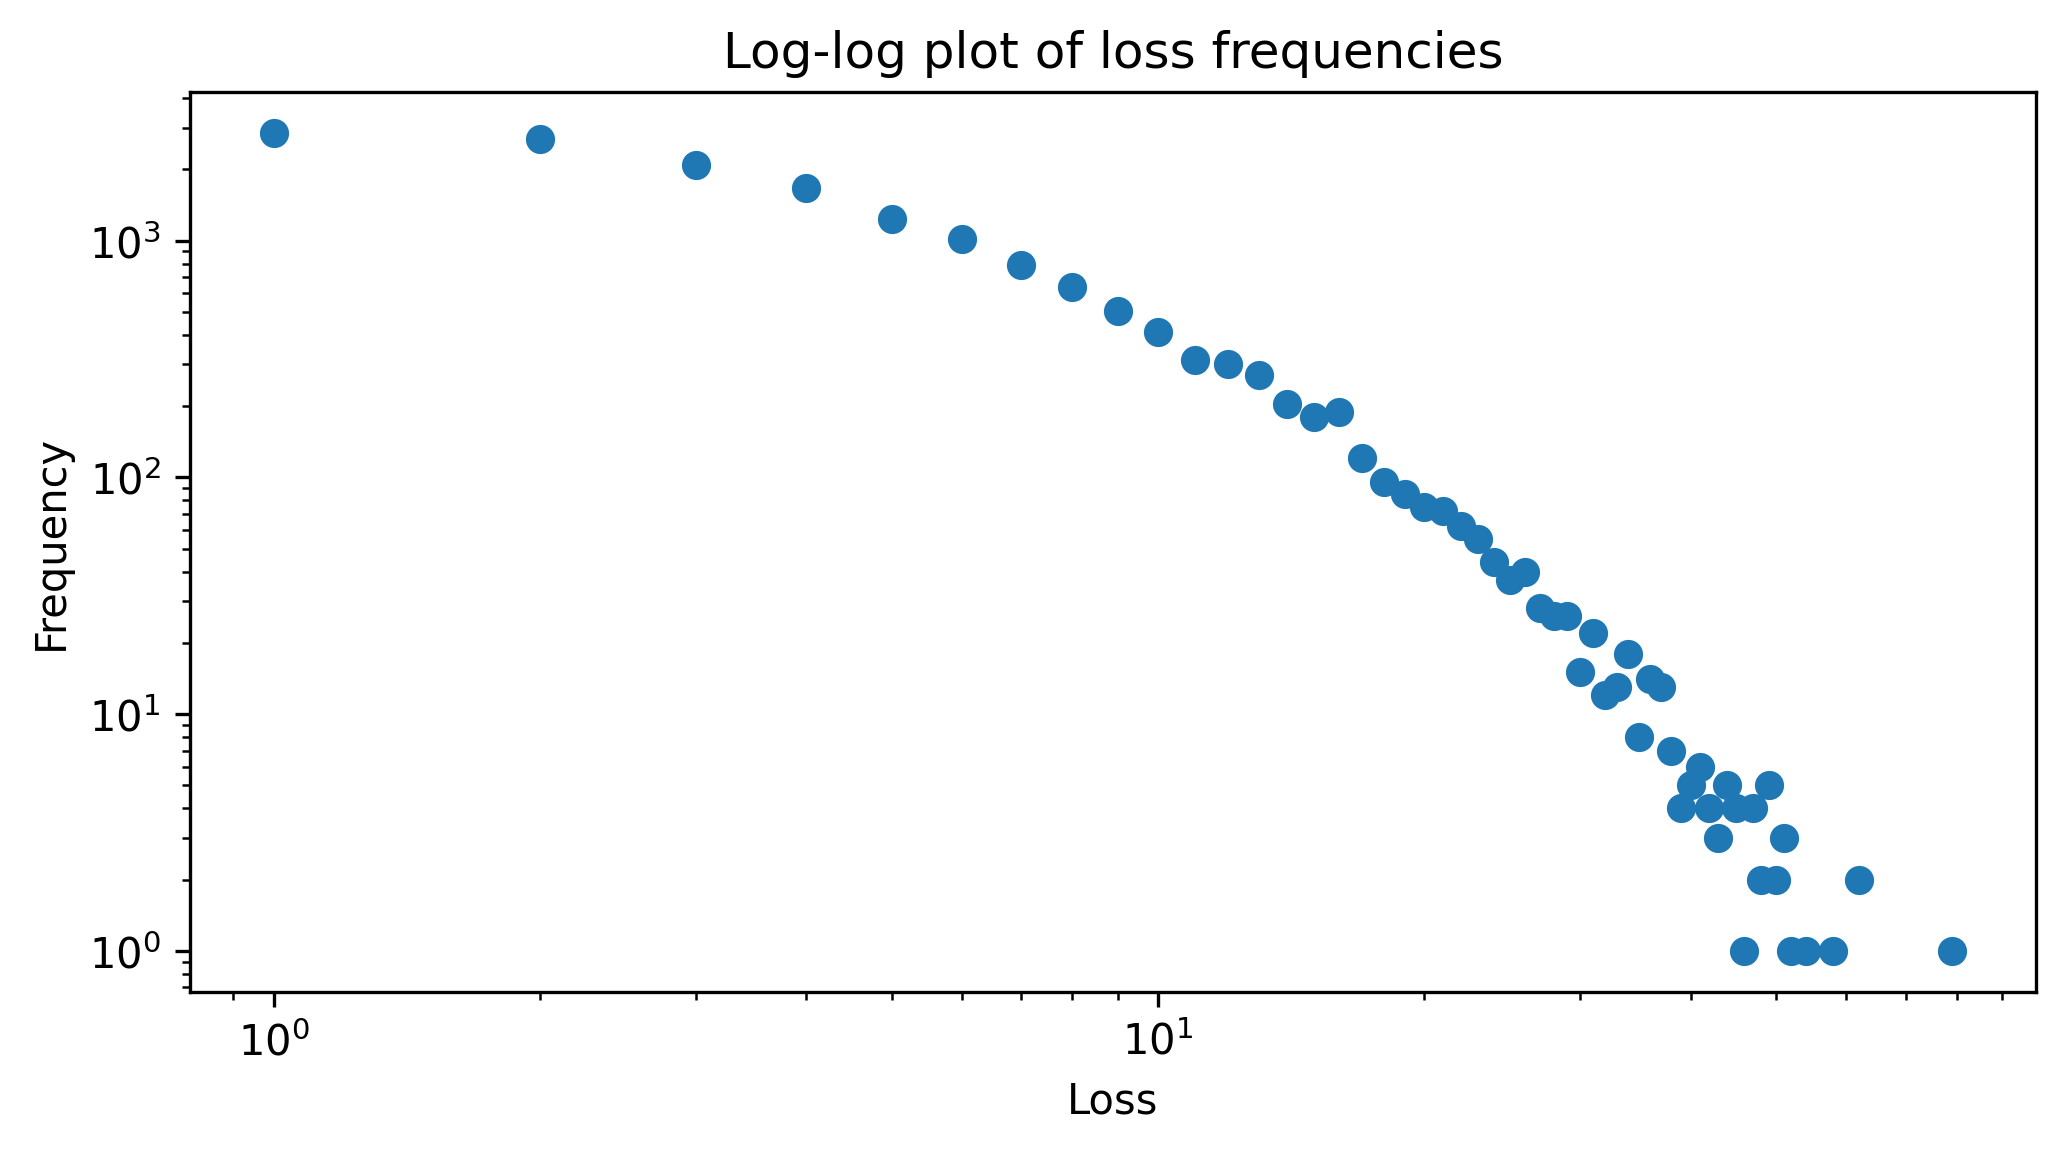
\includegraphics[width=0.45\textwidth]{figures/loss_loglog.png}
    \hfill
    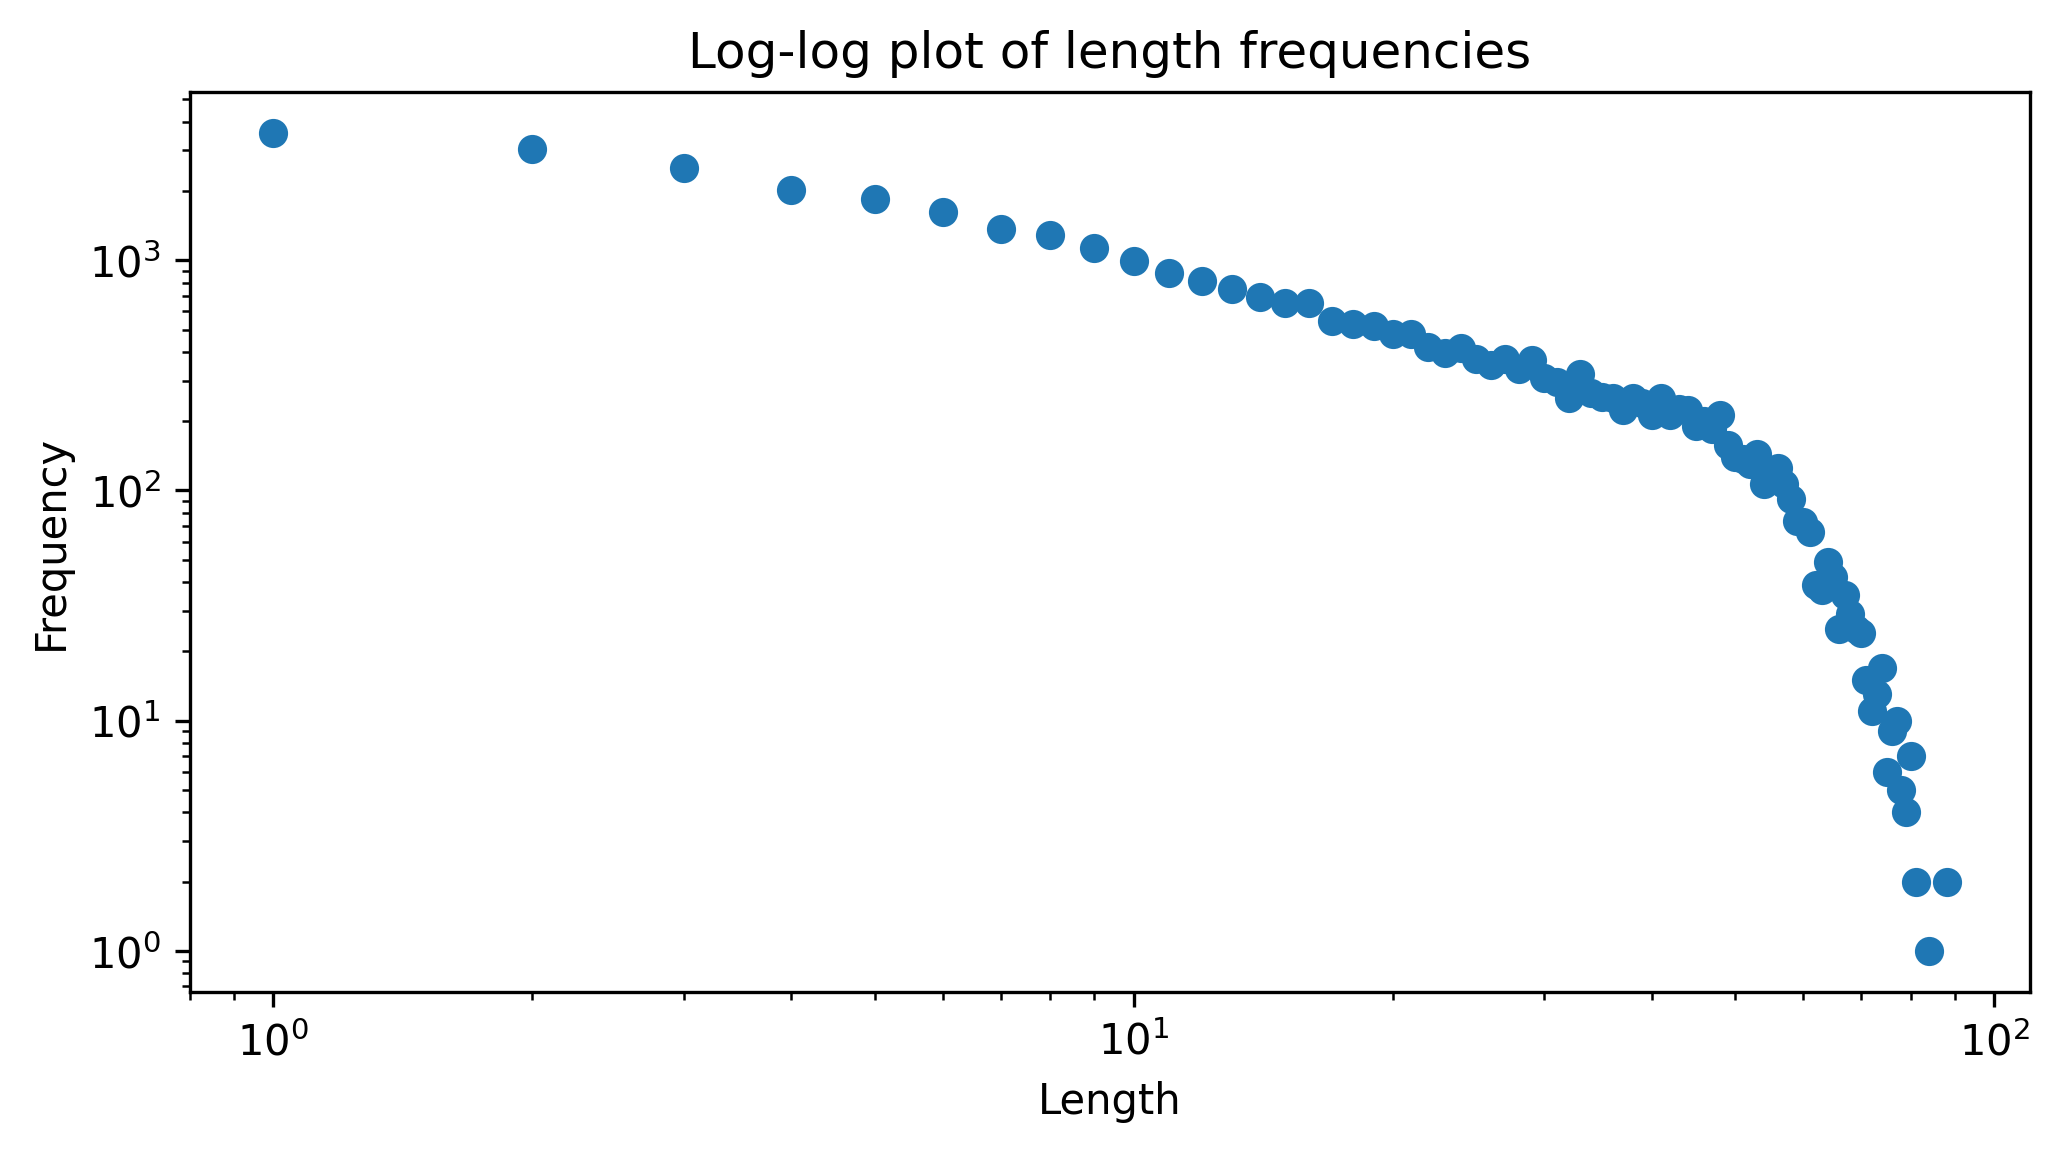
\includegraphics[width=0.45\textwidth]{figures/length_loglog.png}

    \caption{Log--log plots of the avalanche distributions. Approximately linear behaviour
    in the intermediate region suggests power-law behaviour, especially for topples and area.}
    \label{fig:q7_loglog}
\end{figure}

The distributions are not perfect power laws across the whole range. For very small
avalanches, discreteness effects are important because the observables take small integer
values. For very large avalanches, the finite lattice size imposes a cutoff, since an avalanche
cannot spread beyond the boundary of the grid. Thus the power-law behaviour is expected
only in an intermediate scaling region.

The loss distribution is less clean than the distributions for topples and area. This is because
many avalanches do not reach the boundary, so they lose no grains. Positive loss only occurs
when an avalanche reaches the edge of the lattice. Therefore, the loss distribution is more
strongly affected by the boundary condition and the finite size of the system.

The length distribution is also heavy-tailed, but it has a clear finite-size cutoff. This is
expected because the maximum possible avalanche length is limited by the dimensions of
the lattice. Hence the length distribution may only show approximate power-law behaviour
over a restricted intermediate range.

\subsection{Estimated Form of the Distributions}

The results may be summarised as follows:

\begin{table}[htbp]
    \centering
    \begin{tabular}{c|c|p{0.45\textwidth}}
        \hline
        Quantity & Observed distribution & Comment \\
        \hline
        Topples & Approximate power law & The log--log plot has a clear decreasing approximately linear region. \\
        Area & Approximate power law & Similar to topples, with strong evidence of scale-free behaviour. \\
        Loss & Heavy-tailed, less clean & Strongly affected by boundary loss and many zero-loss avalanches. \\
        Length & Heavy-tailed with cutoff & Limited by the finite size of the lattice. \\
        \hline
    \end{tabular}
    \caption{Summary of the avalanche distributions observed in the simulation.}
    \label{tab:q7_distribution_summary}
\end{table}

If a straight-line fit is applied to the approximately linear region of each log--log plot, then
the power-law exponent can be estimated from the fitted slope. If the fitted line is
\[
\log P(x) = a + b \log x,
\]
then
\[
\alpha = -b.
\]
Only the intermediate region should be used for this fit, because the small-avalanche region
is affected by discreteness and the large-avalanche region is affected by finite-size cutoff.

Overall, the avalanche statistics provide evidence that the BTW sandpile model exhibits
self-organized criticality. The model produces many small avalanches and a few large
avalanches, with approximately power-law behaviour in the avalanche observables. This
indicates scale invariance and shows that the system does not have a characteristic
avalanche size.

It remains to find a fit for the exponent.

\section{Abelian Property of the BTW Model}
\label{sec:abelian_property}

The Bak--Tang--Wiesenfeld model has an important mathematical property: the order of
topplings does not affect the final stable configuration. This is called the \textbf{Abelian
property}. To describe this more carefully, we introduce the toppling matrix and toppling
operator.

Let \(\Lambda\) be a finite subset of \(\mathbb{Z}^d\), representing the lattice. In this project,
we mainly consider the two-dimensional case \(d=2\). A sandpile configuration is a function
\[
h : \Lambda \to \mathbb{N}_0,
\]
where \(h(x)\) is the number of grains of sand at the lattice site \(x \in \Lambda\).

A configuration is called \textbf{stable} if
\[
h(x) < z_c
\qquad
\text{for all } x \in \Lambda,
\]
where \(z_c\) is the stability threshold. A configuration is \textbf{unstable} if there exists at
least one site \(x \in \Lambda\) such that
\[
h(x) \geq z_c.
\]

For the two-dimensional BTW model, the threshold is
\[
z_c = 4,
\]
because a site topples when it has four or more grains.

\subsection{Question 9: Conditions on the Toppling Matrix}

The toppling matrix \(\Delta(x,y)\) describes how sand is redistributed when the site \(x\)
topples. The project gives the following conditions:
\[
\forall x,y \in \Lambda,\ x \neq y, 
\qquad
\Delta(x,y)=\Delta(y,x) \geq 0,
\tag{4a}
\]
\[
\forall x \in \Lambda,
\qquad
\Delta(x,x)<0,
\tag{4b}
\]
\[
\forall x \in \Lambda,
\qquad
\sum_{y \in \Lambda} \Delta(x,y) \leq 0,
\tag{4c}
\]
and
\[
\sum_{x,y \in \Lambda} \Delta(x,y) < 0.
\tag{4d}
\]

Condition \((4a)\) says that, for two different sites \(x\) and \(y\), the amount of sand
transferred between neighbouring sites is non-negative and symmetric. The non-negativity
is natural because a toppling should add grains to neighbouring sites, not remove grains
from them. The symmetry condition means that the interaction between sites is undirected:
if \(x\) is a neighbour of \(y\), then \(y\) is also a neighbour of \(x\).

Condition \((4b)\) says that
\[
\Delta(x,x)<0.
\]
This means that when site \(x\) topples, it loses grains. This is necessary because toppling
is supposed to reduce the height of an unstable site. In the two-dimensional BTW model,
the toppled site loses four grains, so \(\Delta(x,x)=-4\).

Condition \((4c)\) says that the total change in the amount of sand caused by toppling one
site is less than or equal to zero:
\[
\sum_{y \in \Lambda} \Delta(x,y) \leq 0.
\]
This means that a toppling cannot create sand overall. In the interior of the lattice, the sum
is equal to zero because the four grains lost by \(x\) are transferred to its four neighbours.
At the boundary, some grains may leave the lattice, so the sum is negative.

Condition \((4d)\) says that
\[
\sum_{x,y \in \Lambda} \Delta(x,y) < 0.
\]
This ensures that the system is dissipative overall. In other words, somewhere in the lattice
there must be a possibility for sand to leave the system. This is important for the model to
reach a statistically stationary state. Without dissipation, sand would keep accumulating
and the system would not stabilize in the same way.

\subsection{Question 10: The BTW Toppling Matrix}

In the BTW model, the toppling matrix is defined by
\[
\Delta(x,y)
=
\begin{cases}
-2d, & x=y, \\
1, & x \text{ and } y \text{ are nearest neighbours}, \\
0, & \text{otherwise}.
\end{cases}
\]
In the two-dimensional case, \(d=2\), so this becomes
\[
\Delta(x,y)
=
\begin{cases}
-4, & x=y, \\
1, & x \text{ and } y \text{ are nearest neighbours}, \\
0, & \text{otherwise}.
\end{cases}
\]

This definition exactly represents the BTW toppling rule. When a site \(x\) topples, it loses
four grains:
\[
h(x) \mapsto h(x)-4.
\]
Each of its four nearest neighbours receives one grain:
\[
h(y) \mapsto h(y)+1
\]
whenever \(y\) is a nearest neighbour of \(x\).

We now verify that this matrix satisfies the four conditions.

First, if \(x \neq y\), then
\[
\Delta(x,y)=1
\]
when \(x\) and \(y\) are nearest neighbours, and otherwise
\[
\Delta(x,y)=0.
\]
Thus
\[
\Delta(x,y) \geq 0.
\]
Also, the nearest-neighbour relation is symmetric, so
\[
\Delta(x,y)=\Delta(y,x).
\]
Therefore condition \((4a)\) is satisfied.

Second, for every site \(x\),
\[
\Delta(x,x)=-4<0.
\]
Therefore condition \((4b)\) is satisfied.

Third, consider the row sum
\[
\sum_{y \in \Lambda} \Delta(x,y).
\]
If \(x\) is an interior site, then it has four nearest neighbours inside the lattice. Hence
\[
\sum_{y \in \Lambda} \Delta(x,y)
=
-4+1+1+1+1
=
0.
\]
If \(x\) is a boundary site, then it has fewer than four neighbours inside the lattice. For
example, an edge site has three neighbours and a corner site has two neighbours. Therefore
the row sum is negative:
\[
-4+3=-1
\]
for an edge site, and
\[
-4+2=-2
\]
for a corner site. Hence, in all cases,
\[
\sum_{y \in \Lambda} \Delta(x,y) \leq 0.
\]
So condition \((4c)\) is satisfied.

Finally, because the lattice has boundary sites, there are sites for which the row sum is
strictly negative. Therefore,
\[
\sum_{x,y \in \Lambda} \Delta(x,y) < 0.
\]
This verifies condition \((4d)\). The strict negativity comes from grains being lost when
boundary sites topple.

Thus the BTW toppling matrix satisfies all the required conditions. The stability threshold
in the two-dimensional BTW model is
\[
z_c=4.
\]

\subsection{Question 11: Commutativity of Toppling Operators}

Using the toppling matrix, we define the toppling operator \(T_x\). If \(x\) is unstable, then
toppling at \(x\) maps a configuration \(h\) to a new configuration \(T_x h\), where
\[
(T_xh)(y)
=
h(y)+\Delta(x,y).
\]
In other words, toppling at \(x\) adds the row \(\Delta(x,\cdot)\) of the toppling matrix to
the height configuration.

More explicitly, in the two-dimensional BTW model,
\[
(T_xh)(x)=h(x)-4,
\]
and if \(y\) is a nearest neighbour of \(x\), then
\[
(T_xh)(y)=h(y)+1.
\]
All other sites are unchanged.

Now suppose that \(x\) and \(x'\) are both unstable sites in the configuration \(h\). We want
to show that the toppling operators commute:
\[
T_xT_{x'}h = T_{x'}T_xh.
\]

For any site \(y \in \Lambda\), first topple \(x'\), then topple \(x\). We get
\[
(T_xT_{x'}h)(y)
=
(T_{x'}h)(y)+\Delta(x,y).
\]
Since
\[
(T_{x'}h)(y)=h(y)+\Delta(x',y),
\]
we have
\[
(T_xT_{x'}h)(y)
=
h(y)+\Delta(x',y)+\Delta(x,y).
\]

On the other hand, if we first topple \(x\), then topple \(x'\), we get
\[
(T_{x'}T_xh)(y)
=
(T_xh)(y)+\Delta(x',y).
\]
Since
\[
(T_xh)(y)=h(y)+\Delta(x,y),
\]
we have
\[
(T_{x'}T_xh)(y)
=
h(y)+\Delta(x,y)+\Delta(x',y).
\]

But addition of integers is commutative, so
\[
h(y)+\Delta(x',y)+\Delta(x,y)
=
h(y)+\Delta(x,y)+\Delta(x',y).
\]
Therefore, for every site \(y \in \Lambda\),
\[
(T_xT_{x'}h)(y)
=
(T_{x'}T_xh)(y).
\]
Hence
\[
T_xT_{x'}h = T_{x'}T_xh.
\]

This proves that toppling operators commute when both topplings are allowed. Therefore,
the order in which unstable sites are toppled does not affect the resulting configuration.
This proves the Abelian property of the BTW sandpile model. Consequently, in the numerical implementation, we do not need to keep track of a unique physically meaningful order of topplings. Instead, all currently unstable sites can be stored in a queue and processed one by one. Although the queue imposes some computational order, the Abelian property guarantees that the final stable configuration is independent of this chosen order.
%---------------------------

%---------------------------APPENDICES
\begin{appendices}
 \input{appendix1}
\end{appendices}
%---------------------------

%---------------------------BIBLIOGRAPHY
\addcontentsline{toc}{chapter}{Bibliography}
\bibliographystyle{abbrv}
\bibliography{biblio}
%---------------------------

\end{document}